\section{Integer Linear Programming Approach}
In the ILP approach, we represent the feasible solution $x$ of the allocation problem as a 3-dimensional binary matrix, where $x^k_{ij}$ refers to the allocation of a software component $c^k_i$ on node $m_j$, $c^k$ refers to the $k^{th}$ replica of $c$. For the running example, a particular feasible solution is shown in Figure \ref{fig_matrix_feasible_solution}.


\begin{center}


\begin{equation*}
\textbf{$\textbf{x}$}=
\begin{bmatrix} 

%first element
\begin{minipage}{.3\textwidth}
\centering
\[
\begin{bmatrix} 
x_{11}^1 & x_{12}^1 & \dots & x_{1J}^1\\
x_{21}^1 & x_{22}^1 & \dots & x_{2J}^1\\
\vdots & \vdots & \ddots & \vdots\\
x_{I1}^1 & x_{I2}^1 & \cdots & x_{IJ}^1
\end{bmatrix}
\]
%second element
\end{minipage}~
\begin{minipage}{0.3\textwidth}
\centering
\[
\begin{bmatrix} 
x_{11}^2 & x_{12}^2 & \dots & x_{1J}^2\\
x_{21}^2 & x_{22}^2 & \dots & x_{2J}^2\\
\vdots & \vdots & \ddots & \vdots\\
x_{I1}^2 & x_{I2}^2 & \cdots & x_{IJ}^2
\end{bmatrix}
\]
\end{minipage}
% dots
...
%last element
\begin{minipage}{0.3\textwidth}
\centering
\[
\begin{bmatrix} 
x_{11}^K & x_{12}^K & \dots & x_{1J}^K\\
x_{21}^K & x_{22}^K & \dots & x_{2J}^K\\
\vdots & \vdots & \ddots & \vdots\\
x_{I1}^K & x_{I2}^K & \cdots & x_{IJ}^K
\end{bmatrix}
\]
\end{minipage}

\end{bmatrix}
\end{equation*}

\captionof{figure}{A Feasible Solution $x$ for K=2.}
\label{fig_matrix_feasible_solution}
\end{center}
% \begin{center}
% \begin{minipage}{.4\textwidth}
% \centering
% \begin{equation}
% \textbf{x$^0$}=
% \begin{bmatrix} 
% 0 & 1 & 0\\
% 1 & 0 & 0\\
% 0 & 1 & 0\\
% 0 & 1 & 0\\
% 0 & 1 & 0
% \end{bmatrix}
% \end{equation}
% \end{minipage}~
% \begin{minipage}{0.4\textwidth}
% \centering
% \begin{equation}
% \textbf{x$^1$}=
% \begin{bmatrix} 
% 0 & 0 & 1\\
% 0 & 1 & 0\\
% 0 & 0 & 1\\
% 0 & 0 & 1\\
% 0 & 0 & 1
% \end{bmatrix}
% \end{equation}
% \end{minipage}
% \captionof{figure}{A Feasible Solution $x$ for K=2.}
% \label{fig_matrix_feasible_solution}
% \end{center}

\subsection{Objective Function}
The power consumption $p(x)$ is computed as the sum of the average power consumption of individual nodes $p_m(x)$ by using Equation \ref{eqn_avgpowerconsumption_util}, where $p_m(x)$ is computed first using Equation x, with utilization of the node $u_m$ as its argument, which is calculated using Equation \ref{lbl_util}as the sum of the utilization of the components (including the replicas) allocated to that node. A component's utilization is obtained from the sum of the utilization of the tasks that realize the component's functionality using Equation \ref{eqn_util_component}.

\begin{align}
\label{eqn_avgpowerconsumption_util}
p(x) = \sum\limits_{m\in M}{p_{m}(x)}&\\
\label{lbl_power}
p_{m}(x) = f_p(u_{m}{(x)})&\\
\label{lbl_util}
u_{m}{(x)} = \sum_k{\sum_i{u_{c_i}*x^k_{ij}}} & \text{ where }j=M^{-1}(m)\\
\label{eqn_util_component}
u_c = \sum_{\tau\in T_{c}} \frac{Exec(\tau_{m})}{Period(\tau)}&
\end{align}

Table \ref{tbl_powerconsumption} illustrates the power consumption calculation of the software allocation example for the feasible solution (\ref{fig_matrix_feasible_solution}).

% Please add the following required packages to your document preamble:
% \usepackage{booktabs}
\begin{table}[h]
\linespread{1.0}\small
\centering
\begin{tabular}{@{}llll@{}}
\toprule
M  & C                             					& $U_c (x)$                                    & $P_m (x)$      \\ \midrule
$m_1$ & {[}$c^1_2${]}                     			& {[}0.046, 0.017{]}                       & 61.155W  \\[0.3em]
$m_2$ & {[}$c^1_1, c^2_2, c^1_3, c^1_4, c^1_5${]} 	& {[}0.196, 0.248, 0.149, & 114.648W \\[0.3em]
		& & 0.091, 0.034{]} &\\[0.3em]
$m_3$ & {[}$c^2_1, c^2_3, c^2_4, c^2_5${]}     		& {[}0.224, 0.137, 0.050{]}                & 131.731W \\[0.3em] \bottomrule
& & Total Power Consumption & 307.534W\\
\end{tabular}
\caption{Average and Total Power Consumption of Nodes.}
\label{tbl_powerconsumption}
\end{table}

In the ideal case, the minimum power consumption of the distributed system is achieved by centralizing the application on fewer nodes. However, due to the timing and reliability constraints, which require additional computing resources, the optimal solution could result in more used nodes. 

\subsection{Constraints}
\paragraph{Software Application Reliability Constraint}
An optimal solution $x$ must fulfill the application reliability requirement RelReq, which is usually in the range [$0.999, 0.999999$] for safety-critical applications. The ILP formulation of the application reliability model, which is shown in (\ref{eqn_appreliability}), is shown in (\ref{eqn_appreliability_milp}).
\begin{align}
\label{eqn_appreliability_milp}
Reliability(x)=\sum_{s\in PS}[f(x,s)]*p_s,
\end{align}
where $[f(x,s)]$ is an \textit{Iverson function } that returns $0$ if the proposition that the application functions in state $s$ is \textit{true}. Otherwise it returns $1$ if the proposition that application functions in state $s$ is \textit{false} (or the application fails in state $s$ is \textit{true}). The application functions only if all of its constituent software components functions and fails if at least of one of its components fails as formulated in (\ref{eqn_appreliability_milp_components}), via the floor function. A software component functions if there exists a node $m_j$ that hosts the component's replica $x_{ij}^k=1$ and at the same time the node functions $s_{j}=1$, which is formulated in (\ref{eqn_appreliability_milp_component}) via the ceiling function. The floor and ceiling functions are piecewise linear functions, and are linearized by the ILP solver.

\begin{align}
f(x,s) = \floor[\Bigg]{\frac{\sum_if_{c_i}(x,s)}{N}}=
\begin{cases}
1 & \mbox{if } application \mbox{ functions}\\
0 & \mbox{if } application \mbox{ fails}
\end{cases}\label{eqn_appreliability_milp_components}\\
f_{c_i}(x,s) = \ceil[\Bigg]{\frac{\sum_k\sum_j x^{k}_{ij}*s_j}{K}}=
\begin{cases}
1 & \mbox{if } c_i \mbox{ functions}\\
0 & \mbox{if } c_i \mbox{ fails}
\end{cases}\label{eqn_appreliability_milp_component}
\end{align}

Table \ref{tbl_application_rel} demonstrates the application reliability calculation for the feasible solution $x$ (\ref{fig_matrix_feasible_solution}). %Figure~\ref{fig_comp_replications} shows pictorial descriptions of component allocations on nodes with no replication $K=1$, and with replications $K=2$. 
\begin{table}[h]
\centering
\begin{tabular}{@{}llll@{}}
\toprule
$s$   & $p_s$     & {[}$f_{c_i}(x), i=1,2,3,4${]} & $f_a(x)$ \\ \midrule
000 & 0.0000000000 & {[}0, 0, 0, 0{]}          & 0     \\
001 & 0.0000000099 & {[}0, 0, 0, 1{]}          & 0     \\
010 & 0.0000000099 & {[}1, 1, 1, 1{]}          & 1     \\
011 & 0.0000999800 & {[}1, 1, 1, 1{]}          & 1     \\
100 & 0.0000000099 & {[}1, 1, 1, 0{]}          & 0     \\
101 & 0.0000999800 & {[}1, 1, 1, 0{]}          & 0     \\
110 & 0.0000999800 & {[}1, 1, 1, 1{]}          & 1     \\
111 & 0.9997000299 & {[}1, 1, 1, 1{]}          & 1     \\ \bottomrule
\end{tabular}
\caption{Application Reliability Calculation using State Enumeration Method, R(x) = 0.9998999998.}
\label{tbl_application_rel}
\end{table}

% \begin{figure}
%     \centering
%     \begin{subfigure}[b]{0.2\textwidth}
%         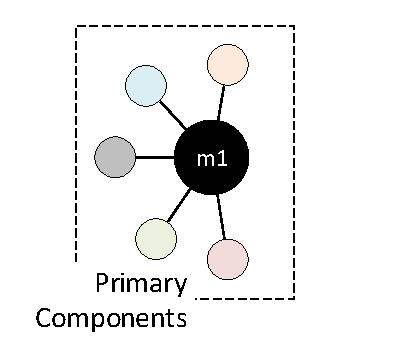
\includegraphics[width=\textwidth]{k0}
%         \caption{No replication, K = 1.}
%         \label{fig:datachainsingle}
%     \end{subfigure}
%     ~ %add desired spacing between images, e. g. ~, \quad, \qquad, \hfill etc. 
%       %(or a blank line to force the subfigure onto a new line)
%     \begin{subfigure}[b]{0.25\textwidth}
%         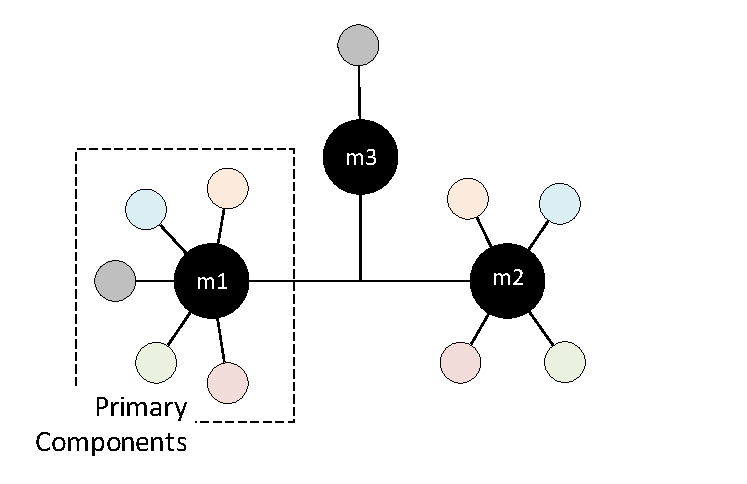
\includegraphics[width=\textwidth]{k1}
%         \caption{With replication, K = 2.}
%         \label{fig:datachainmulti}
%     \end{subfigure}
% %     ~
% %         \begin{subfigure}[b]{0.3\textwidth}
% %         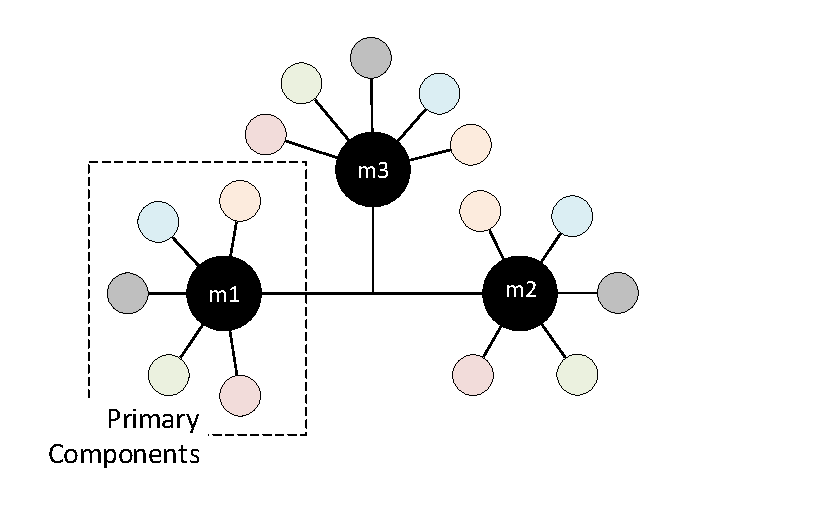
\includegraphics[width=\textwidth]{k2}
% %         \caption{With Replication, K = 3}
% %         \label{fig:datachainsingle}
% %     \end{subfigure}
%     \caption{Allocation of Components.}
%     \label{fig_comp_replications}
% \end{figure}

In the case that the application reliability could be met with less replications, there is no need to keep unnecessary component replicas in the system. To this end, our optimization algorithm imposes soft constraints for $k>1$, which implies that replicas allocated on the same node are reduced to a single replica, essentially discarding the extra replicas by design, since the reliability does not improve following additional replicas on the same node, assuming our fault model.

\paragraph{Timing Constraints}
The timing constraints ensure that the response times of the tasks realizing the distributed application meet their deadlines. Furthermore, they ensure that the cause-effect chains satisfy their respective end-to-end timing requirements, for all possible failure-modes of the system. The constraints are formulated as logical constraints in the ILP problem, as explained in the rest of this subsection.

\paragraph*{Tasks Deadline Constraints}
The following pseudo-code illustrates how the ILP logical constraints of the tasks deadlines are prepared. It explores all possible sets of components combinations (or partitions) that can potentially be allocated to a node. Only the sets that are schedulable are asserted as constraints of the optimization problem, which is explained as follows: Line (1) identifies the power set of the components $Par$, followed by synthesis of tasks models of each partition. Line (2) checks the tasks models' schedulability and returns a matrix $M^T$ that indicates schedulability, which is \textit{true} if the task model is schedulable and \textit{false} if not schedulable. Line (3) generates an ILP partition expression $E$ for each node, then Line (4-6) asserts the expressions to hold in the optimization for the partitions that are schedulable.
\begin{algorithm}
\SetKwData{Particles}{Particles}
\SetKwInOut{Input}{input}\SetKwInOut{Output}{output}
\SetKwFunction{AssertOR}{assertOR}
\caption{Generate Task Partitions Constraints.}\label{alg_partition}
% \algsetup{
% linenosize=\small,
% linenodelimiter=.
% }	
%\renewcommand{\algorithmicrequire}{\textbf{Input:}}
%\renewcommand{\algorithmicensure}{\textbf{Output:}}
%\begin{algorithmic}[1]
\Input{$C,M$}
\Output{Optimization Satisfies Tasks Deadlines, $D$}
$Par \Leftarrow 2^C$\;	
$M^T\Leftarrow isSched(Par, M)$\;
$E\Leftarrow MilpParExp(x)$\;
\ForEach{$m \in M$}{
	\AssertOR{$M^T_m, E_m, true$}
}
\end{algorithm}

In general, the number of potential logical constraints grow exponentially, which is in $2^{|C|}*|M|$. However, the effective logical constraints that are eventually asserted are much lower, for two main reasons: 1) a portion of the tasks models are not schedulable, therefore eliminated from the power set, due to CPU utilization exceeding the bound, hence not satisfying the response time of either task in the partition; ii) a task model can be a super set of other tasks model. In this case, only the super model is checked, hence reducing pre-optimization time and logical constraints asserted in the solver.

\subsubsection*{Cause-effect Chains Constraints}
These constraints ensure that the cause-effect chains $\Gamma$ meet their respective end-to-end requirements $\mathrm{E2eReq}$. Similar to the previous constraints, the cause-effect chain constraints are logical assertions, which must be fulfilled by the optimal solution. The following pseudo-code illustrates how the ILP logical assertions are synthesized from the input models. 
The pseudo-code contains three main parts: i) the first part in Line (2) identifies the different deployment cases of the cause-effect chains over a set of nodes $M$, ii) the second part in Line (3-5), checks the schedulability of a deployable cause-effect chain $\phi$ against the reaction or age delays  \cite{mubeen2013support} and returns its schedulability matrix $M^\Gamma$, with values $true$ if schedulable and $false$ if not schedulable. For a schedulable $\phi$, Line (5) constructs a conjunctive ILP expression that indicates the existence of at least one schedulable $\phi$ that satisfies the end-to-end requirement imposed on $\gamma$, and iii) the last part in Line (7) asserts the ILP logical OR expressions for each $\gamma$.
\begin{algorithm}
\SetKwData{Particles}{Particles}
\SetKwInOut{Input}{input}
\SetKwInOut{Output}{output}
\caption{Generate Constraints on the Cause-effect Chains.}\label{alg_causeeffectchains}
%\begin{algorithmic}[1]
\Input{$\Gamma,M$}
\Output {Optimization Satisfies End-to-end Requirements of Cause-effect Chains}
\ForEach{$\gamma \in \Gamma$}{
    $\Phi\leftarrow Unique(C^{T_\Gamma}_r, M)$ \;
	\ForEach{$\phi \in \Phi$}{
        $M^\Gamma\Leftarrow isSched(\phi, M)$\;
        $depExp\Leftarrow depExp \lor sched(M^\Gamma, true)$\;
    }
	$assert(depExp)$\;
}
%\end{algorithmic}
\end{algorithm}\vspace{-0.2cm}

\subsection{Solving the ILP Problem}
We use IBM ILOG CPLEX Optimizer to solve our proposed ILP model. CPLEX Optimizer is one of the most robust and high-performing linear programming, mixed integer, and quadratic programming solvers in the market. The ILP problem is encoded in Java via the 
